\documentclass[12pt]{article}

\usepackage{answers}
\usepackage{setspace}
\usepackage{graphicx}
\usepackage{enumitem}
\usepackage{multicol}
\usepackage{mathrsfs}
\usepackage[margin=1in]{geometry} 
\usepackage{amsmath,amsthm,amssymb}
\usepackage{hyperref}
 
\newcommand{\N}{\mathbb{N}}
\newcommand{\Z}{\mathbb{Z}}
\newcommand{\C}{\mathbb{C}}
\newcommand{\R}{\mathbb{R}}

\DeclareMathOperator{\sech}{sech}
\DeclareMathOperator{\csch}{csch}
 
\newenvironment{theorem}[2][Theorem]{\begin{trivlist}
\item[\hskip \labelsep {\bfseries #1}\hskip \labelsep {\bfseries #2.}]}{\end{trivlist}}
\newenvironment{definition}[2][Definition]{\begin{trivlist}
\item[\hskip \labelsep {\bfseries #1}\hskip \labelsep {\bfseries #2.}]}{\end{trivlist}}
\newenvironment{proposition}[2][Proposition]{\begin{trivlist}
\item[\hskip \labelsep {\bfseries #1}\hskip \labelsep {\bfseries #2.}]}{\end{trivlist}}
\newenvironment{lemma}[2][Lemma]{\begin{trivlist}
\item[\hskip \labelsep {\bfseries #1}\hskip \labelsep {\bfseries #2.}]}{\end{trivlist}}
\newenvironment{exercise}[2][Exercise]{\begin{trivlist}
\item[\hskip \labelsep {\bfseries #1}\hskip \labelsep {\bfseries #2.}]}{\end{trivlist}}
\newenvironment{solution}[2][Solution]{\begin{trivlist}
\item[\hskip \labelsep {\bfseries #1}]}{\end{trivlist}}
\newenvironment{problem}[2][Problem]{\begin{trivlist}
\item[\hskip \labelsep {\bfseries #1}\hskip \labelsep {\bfseries #2.}]}{\end{trivlist}}
\newenvironment{question}[2][Question]{\begin{trivlist}
\item[\hskip \labelsep {\bfseries #1}\hskip \labelsep {\bfseries #2.}]}{\end{trivlist}}
\newenvironment{corollary}[2][Corollary]{\begin{trivlist}
\item[\hskip \labelsep {\bfseries #1}\hskip \labelsep {\bfseries #2.}]}{\end{trivlist}}
 
\begin{document}

% --------------------------------------------------------------
%                         Start here
% --------------------------------------------------------------

\title{The Riddler Classic - Marathon Problem}%replace with the appropriate homework number
\author{Jaewon Chung %replace with your name
} %if necessary, replace with your course title

\maketitle
%Below is an example of the problem environment
\begin{problem}{(\href{https://fivethirtyeight.com/features/how-hard-is-it-to-find-a-running-buddy/}{538 Link})}
Given $X_1, X_2, \ldots, X_n \stackrel{i.i.d}{\sim} \mathcal{N}(\mu, \sigma^2)$, estimate the number of $n$ such
that the probability of every pair of r.v.s is less than any $s \geq 0$, 
meaing $|X_i - X_j| \leq s$ for all $i\neq j$, is 0.99.
\end{problem}

%Below is the solution environment
\begin{solution}{}
    The problem can be restated as, what is the gap between the order statistics of the $i.i.d$ random variables.

    Below is from an numerical experiment that looks
    at different number of $N$ runners and different values
    of $s$, which is denoted as $\epsilon$.
    \begin{figure}[h]
    \centering
    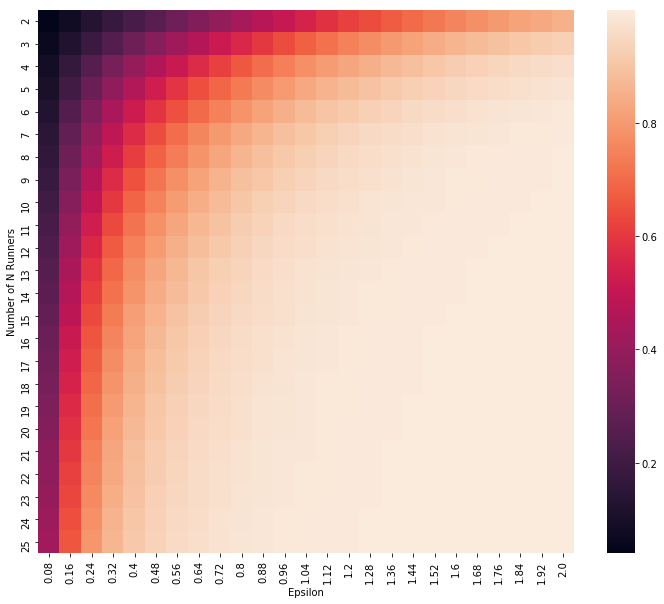
\includegraphics[width=8cm]{heatmap_plot.png}
    \end{figure}
\end{solution}
\end{document}
